\chapter{Análisis de los resultados}
\label{resultados}

A lo largo de este capitulo se va a tratar de analizar, comparar y discutir los resultados obtenidos mediante HFSS sobre los diseños que se comentaron en la sección \ref{analdis}. Se analizará cada configuración por separado y se mostrarán las gráficas y valores principales para cada una de las configuraciones de 2GHz y 6 GHz y finalmente la configuración a 27 GHz. No se analizará el caso del parche simple a 2.4 GHz puesto que ya fue analizado detalladamente en la sección \ref{procesodiseno}.

\section{Parche Simple a 6 GHz}
\par Para el parche simple a 6 GHz los resultados obtenidos son los siguientes:

\subsection{Pérdidas de retorno}
\par Comenzaremos analizando la curva de pérdidas de retorno o parámetro S del parche simple a 6 GHz, donde se puede observar un valor pico de -40.35 dB y un ancho de banda de 168 MHz, desde los 5.917 GHz hasta los 6.086 GHz, lo que equivale a un 2.81\% de la frecuencia de trabajo.
\\
\begin{figure}[H]
    \centering
        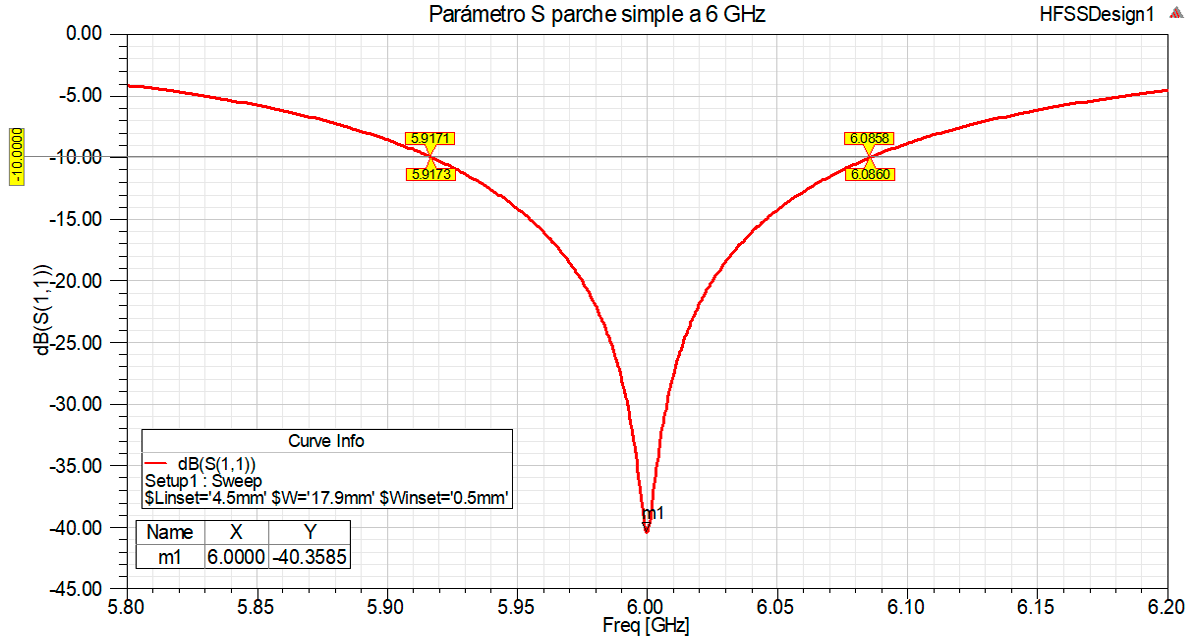
\includegraphics[width=\textwidth]{archivos/analisis/1x12/1}
        \caption{Parámetro S para el parche simple a 6 GHz}
        \label{fig:s1x12}
\end{figure}

\subsection{Reactancia}
\par La curva de reactancia arroja un valor a la frecuencia de trabajo de -0.63 $\Omega$. Muy cerca del valor esperado, 0.
\\
\begin{figure}[H]
    \centering
        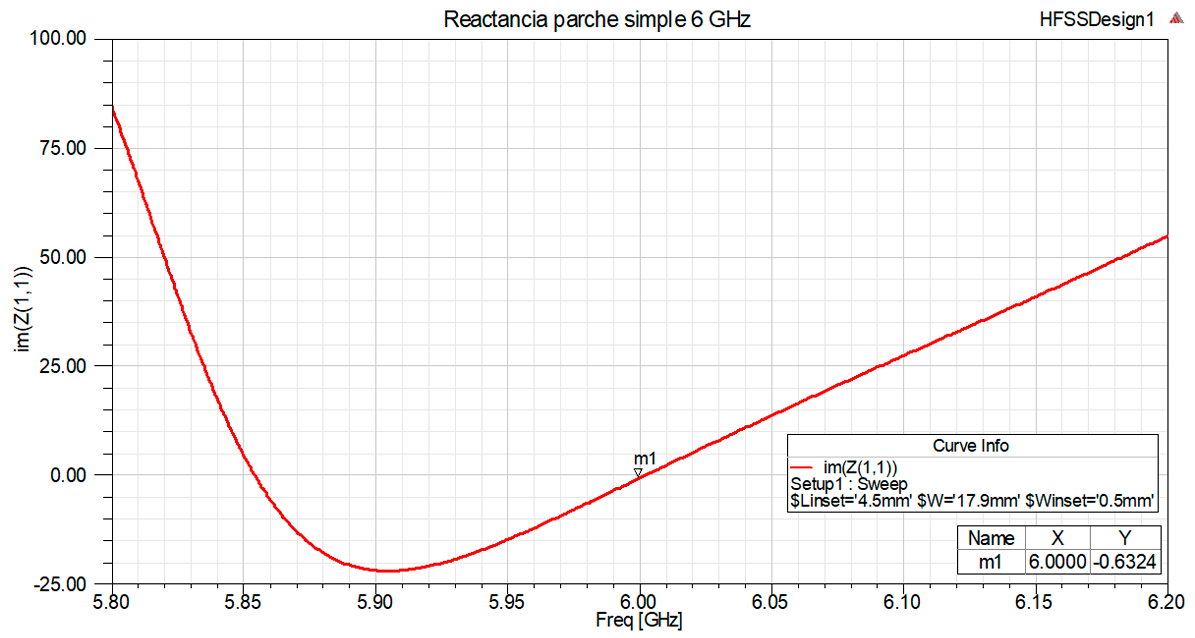
\includegraphics[width=0.85\textwidth]{archivos/analisis/1x12/2}
        \caption{Reactancia para el parche simple a 6 GHz}
        \label{fig:react1x12}
\end{figure}


\subsection{Resistencia}
\par La parte real de la impedancia ofrece un valor a la frecuencia de trabajo de 49.28 $\Omega$. Muy cerca del valor esperado, 50, con un error de tan solo el 1.44\%.
\\
\begin{figure}[H]
    \centering
        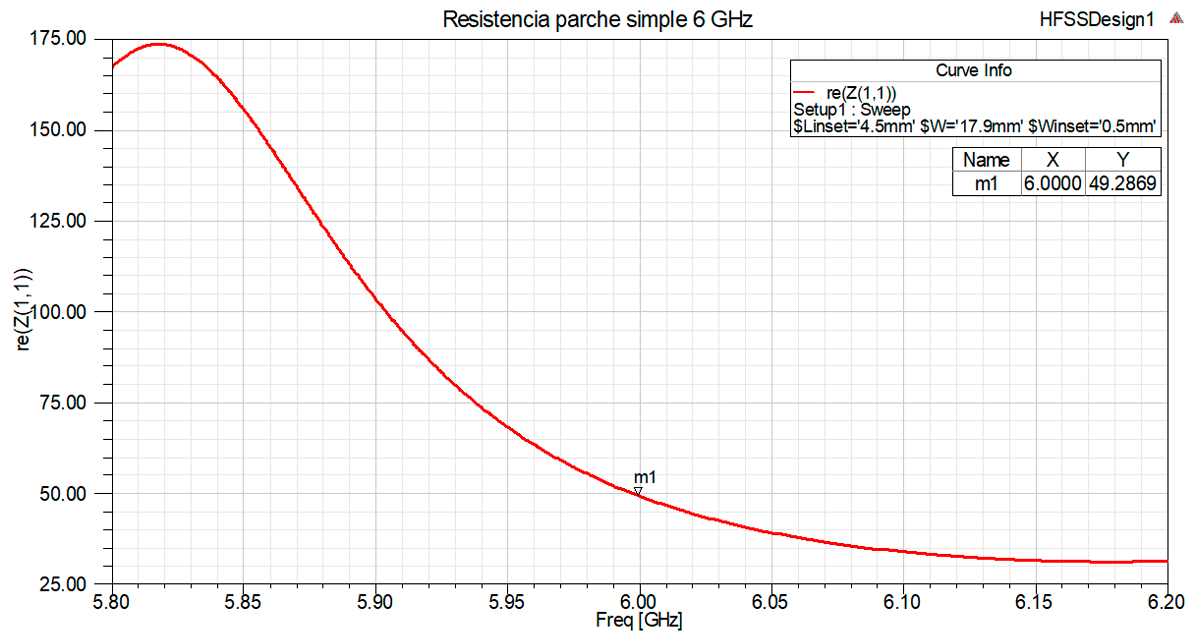
\includegraphics[width=0.85\textwidth]{archivos/analisis/1x12/3}
        \caption{Resistencia para el parche simple a 6 GHz}
        \label{fig:resis1x12}
\end{figure}


\subsection{Patrón de radiación}
\par En cuanto a los patrones de radiación, se puede observar como, al igual que el parche simple a 2.4 GHz, el patrón de radiación es omnidireccional para el plano superior de la antena, y no se ve afectado por ningún otro tipo de elemento radiante. La directividad para el ángulo de máxima radiación encontrada es de 7.66 dB.
\\
\subsubsection{Plano E}
\begin{figure}[H]
    \centering
        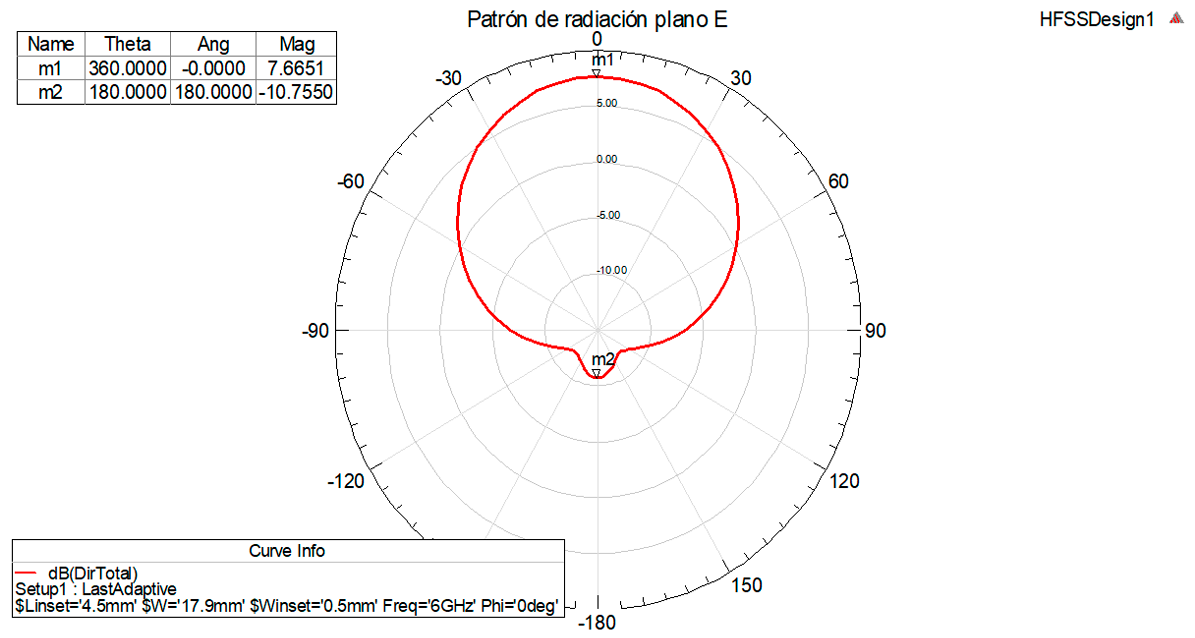
\includegraphics[width=0.8\textwidth]{archivos/analisis/1x12/4}
        \caption{Radiación en el plano E para el parche simple a 6 GHz}
        \label{fig:E1x12}
\end{figure}

\subsubsection{Plano H}
\begin{figure}[H]
    \centering
        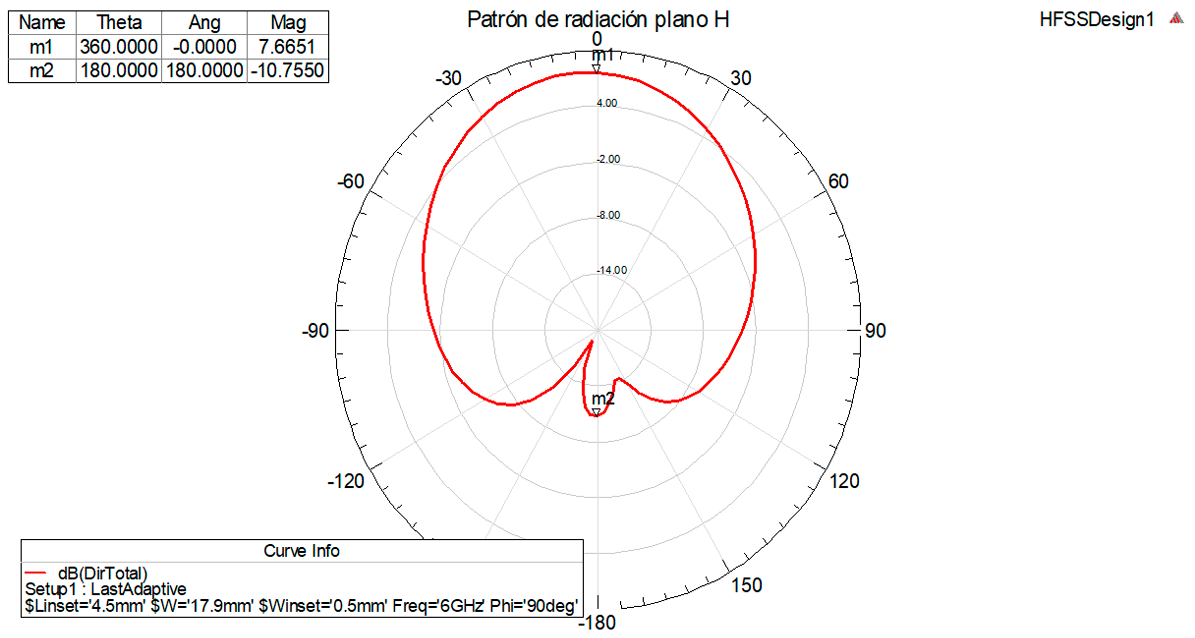
\includegraphics[width=0.8\textwidth]{archivos/analisis/1x12/5}
        \caption{Radiación en el plano H para el parche simple a 6 GHz}
        \label{fig:H1x12}
\end{figure}

\newpage
\subsection{Radiación 3D}
\par Mediante el diagrama de radiación 3D se puede observar el comportamiento omnidireccional de la antena. 

\begin{figure}[H]
     \centering
     \begin{subfigure}[b]{0.75\textwidth}
         \centering
         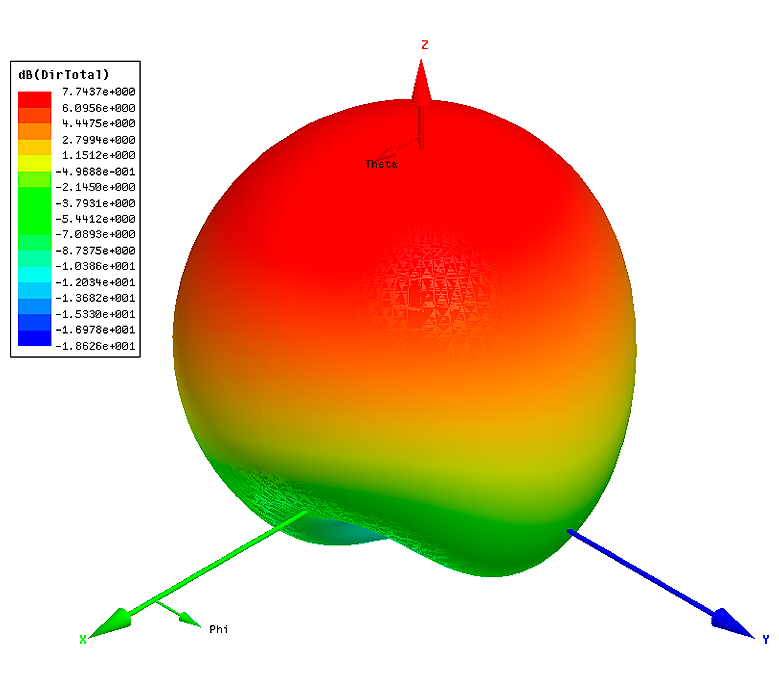
\includegraphics[width=0.85\textwidth]{archivos/analisis/1x12/6}
         \caption{Representación isométrica del diagrama de radiación 3D}
         \label{fig:3d11x12}
     \end{subfigure}
     \hfill
     \begin{subfigure}[b]{0.75\textwidth}
         \centering
         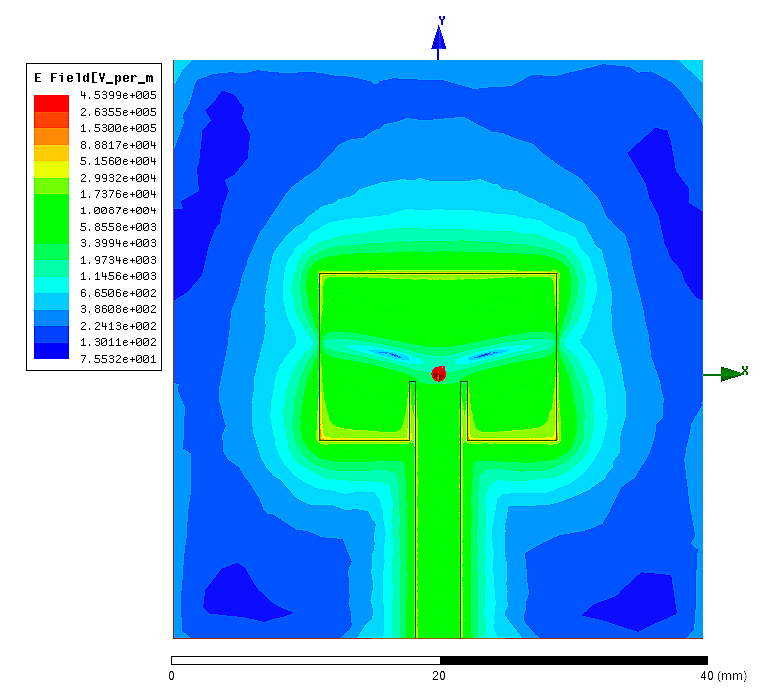
\includegraphics[width=0.85\textwidth]{archivos/analisis/1x12/7}
         \caption{Representación superior del diagrama de radiación 3D}
         \label{fig:3d21x12}
     \end{subfigure}
     \hfill
        \caption{Radiación 3D para el parche simple a 6 GHz}
        \label{fig:3d1x12}
\end{figure}

\newpage
\subsection{Campo eléctrico}
\par Finalmente, podemos observar la distribución de campos eléctricos en el parche. 

\begin{figure}[H]
    \centering
        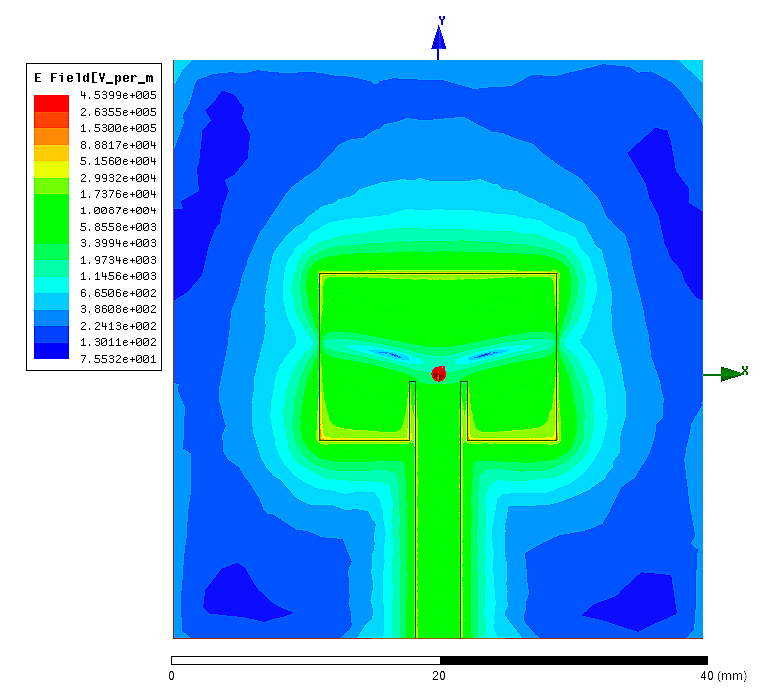
\includegraphics[width=\textwidth]{archivos/analisis/1x12/8}
        \caption{Distribución de campos eléctricos para el parche simple a 6 GHz}
        \label{fig:elec1x12}
\end{figure}


\subsection{Resumen}
\par Como se puede observar en este parche único a 6 GHz, los resultados obtenidos son muy similares a los obtenidos en el caso de 2.4 GHz. El patrón de radiación de la antena se caracteriza por el ser el más básico que podemos encontrar en una antena de tipo microstrip, además de tratarse de un patrón muy útil para aplicaciones móviles puesto que su característica omnidireccional se adapta a los casos de uso en los que el patrón de radiación de la antena no esté apuntando directamente a la antena de telefonía. 
\\
\par En la tabla \ref{tab:1x12} se pueden observar un resumen de los parámetros característicos de la antena. En ella se puede observar el buen rendimiento obtenido

\begin{table}[H]
  
   \label{tab:1x12}
   \small % text size of table content
   \centering % center the table
   \begin{tabular}{m{0.4\linewidth}m{0.4\linewidth}} % alignment of each column data
   \toprule[\heavyrulewidth]\toprule[\heavyrulewidth]
   \textbf{Parámetro} & \textbf{Parche simple 6 GHz} \\ 
   \midrule
   \textbf{S(1,1)} & -40.35 dB \\
   \textbf{Ancho de banda} & 168 MHz dB \\
   \textbf{Directividad} & 7.66 dB \\
   \textbf{Ganancia} & 7.41 dB \\
   \textbf{Eficiencia de radiación} & 93.15\% \\
   \textbf{Relación delante/atrás} & 18.42 dB \\

   \bottomrule[\heavyrulewidth] 
   \end{tabular}
   \caption{Parámetros característicos del parche único microstrip a 6 GHz} 
\end{table}









\section{Array 2x1 a 2.4 GHz}
\par Para el array en configuración 2x1 a 2.4 GHz los resultados obtenidos son los siguientes:

\subsection{Pérdidas de retorno}
\par En cuanto a su curva de pérdidas de retorno del array a 2.4 GHz, se puede observar un valor pico de -36.46 dB y un ancho de banda de 34.3 MHz, desde los 2.3835 GHz hasta los 2.4173 GHz, lo que equivale a un 1.43\% de la frecuencia de trabajo.
\\
\begin{figure}[H]
    \centering
        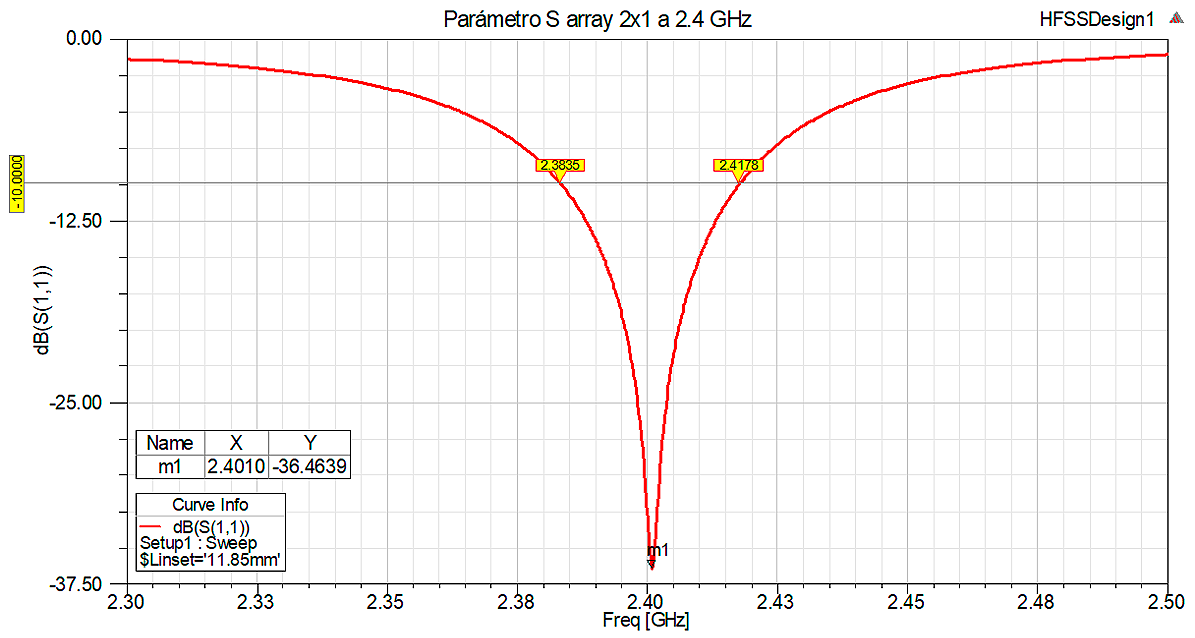
\includegraphics[width=\textwidth]{archivos/analisis/2x11/1}
        \caption{Parámetro S para el array 2x1 a 2.4 GHz}
        \label{fig:s2x11}
\end{figure}

\subsection{Reactancia}
\par La curva de reactancia arroja un valor a la frecuencia de trabajo de -1.37 $\Omega$. 
\\
\begin{figure}[H]
    \centering
        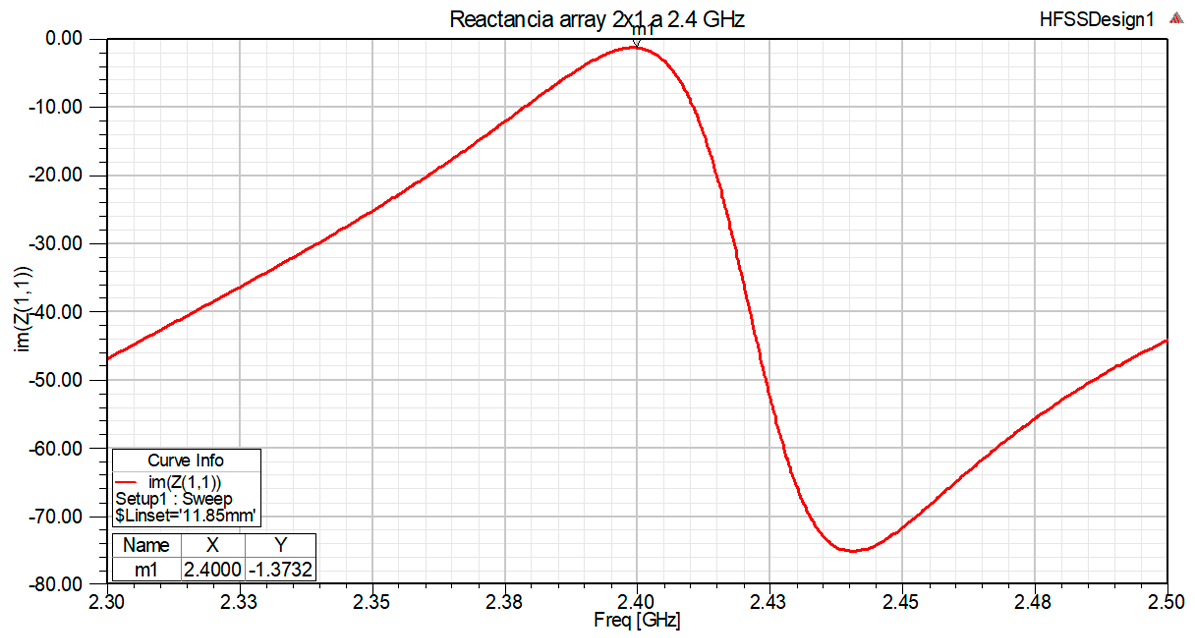
\includegraphics[width=0.85\textwidth]{archivos/analisis/2x11/2}
        \caption{Reactancia para el array 2x1 a 2.4 GHz}
        \label{fig:react2x11}
\end{figure}

\subsection{Resistencia}
\par La parte real de la impedancia ofrece un valor a la frecuencia de trabajo de 48.12 $\Omega$.
\\
\begin{figure}[H]
    \centering
        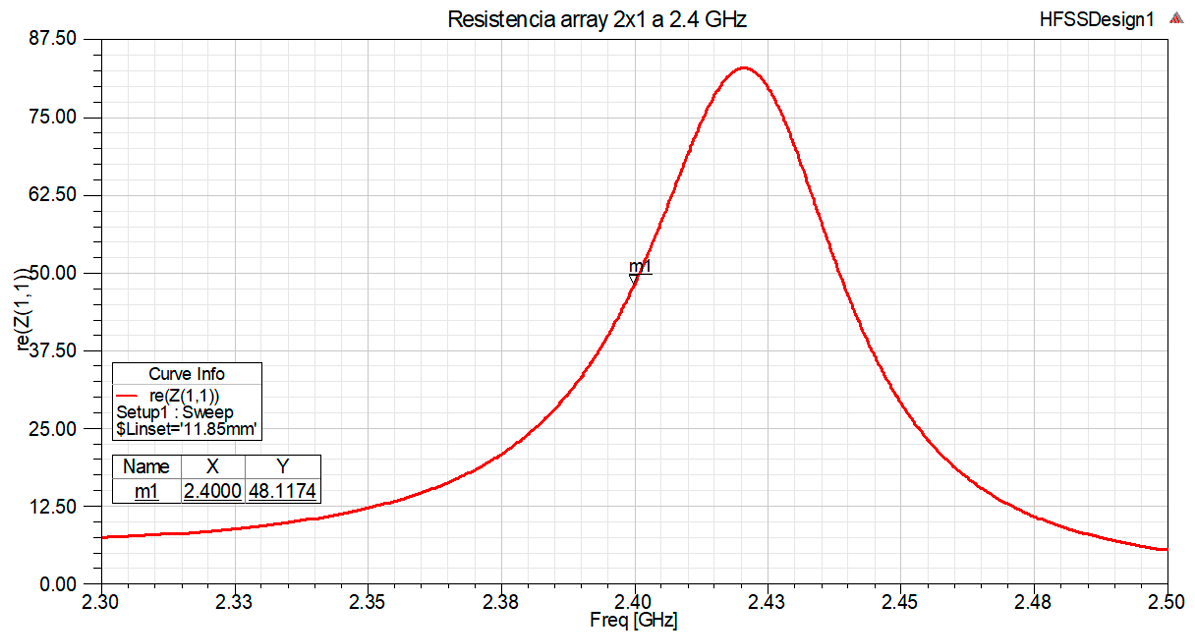
\includegraphics[width=0.85\textwidth]{archivos/analisis/2x11/3}
        \caption{Resistencia para el array 2x1 a 2.4 GHz}
        \label{fig:resis2x11}
\end{figure}

\subsection{Patrón de radiación}
\par En cuanto a los patrones de radiación, se puede observar se puede observar un comportamiento más directivo con unos lóbulos laterales y trasero de bastante magnitud en relación al lóbulo principal para el plano E, mientras que en el plano H se observa un comportamiento completamente omnidireccional para el plano superior del array. La directividad en el ángulo de máxima radiación observada es de 7.64 dB.
\\
\subsubsection{Plano E}
\begin{figure}[H]
    \centering
        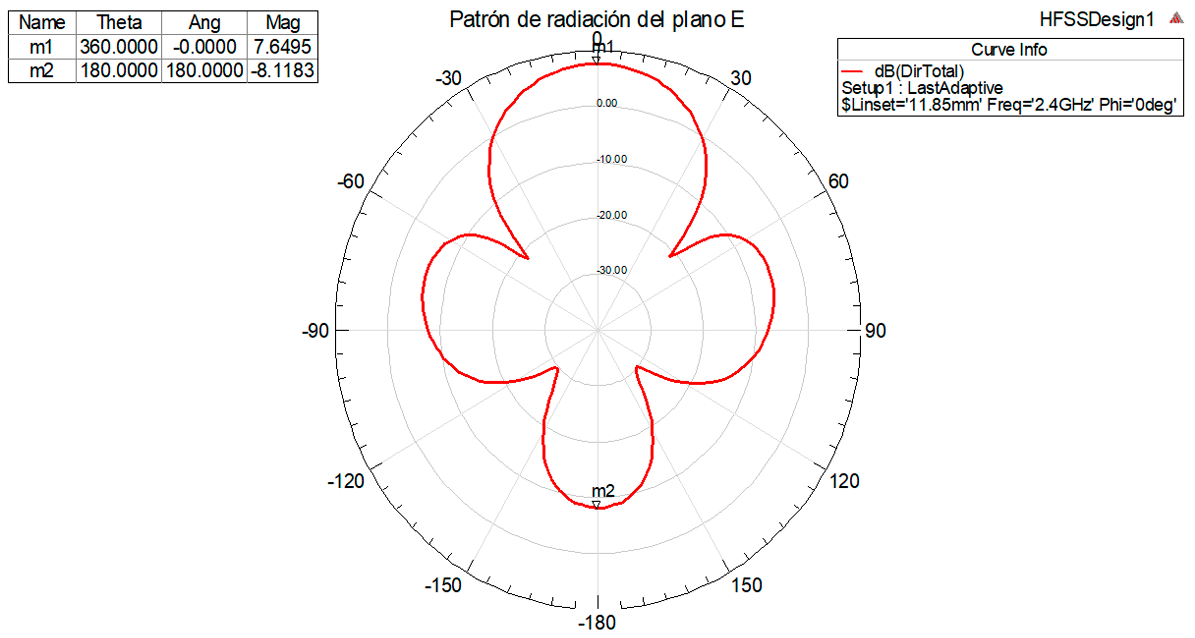
\includegraphics[width=0.75\textwidth]{archivos/analisis/2x11/4}
        \caption{Radiación en el plano E para el array 2x1 a 2.4 GHz}
        \label{fig:E2x11}
\end{figure}

\subsubsection{Plano H}
\begin{figure}[H]
    \centering
        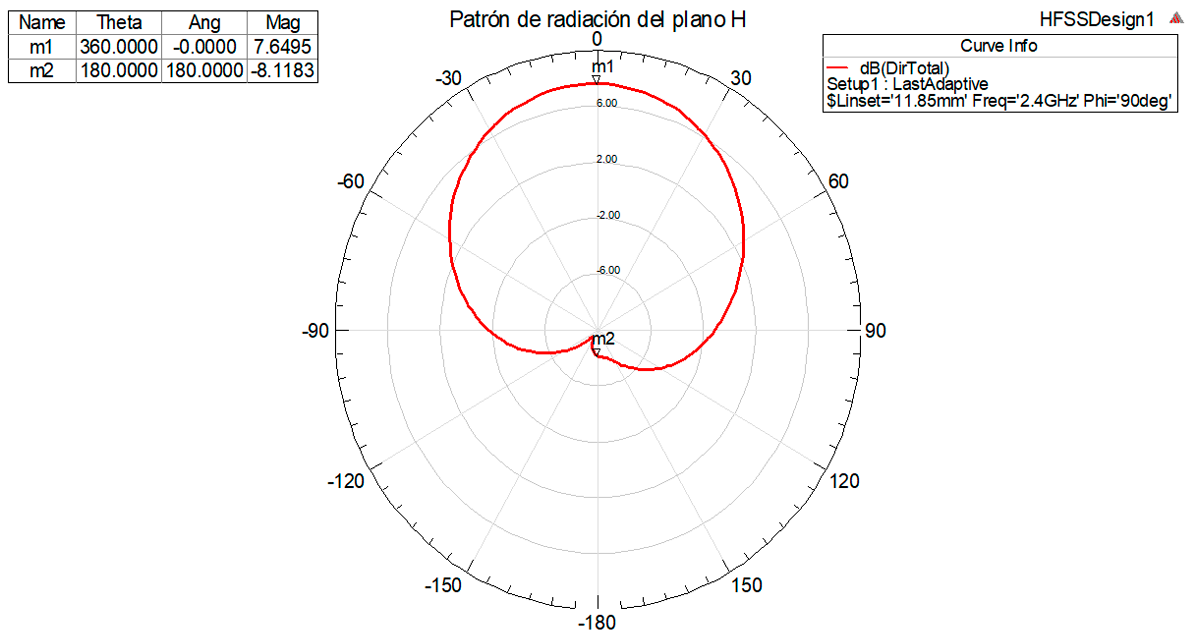
\includegraphics[width=0.75\textwidth]{archivos/analisis/2x11/5}
        \caption{Radiación en el plano H para el array 2x1 a 2.4 GHz}
        \label{fig:H2x11}
\end{figure}

\subsection{Radiación 3D}
\par Mediante el diagrama de radiación 3D se puede observar el comportamiento directivo en el plano perpendicular a la configuración del array, producido por la superposición de la radiación de ambos parches.

\begin{figure}[H]
     \centering
     \begin{subfigure}[b]{0.7\textwidth}
         \centering
         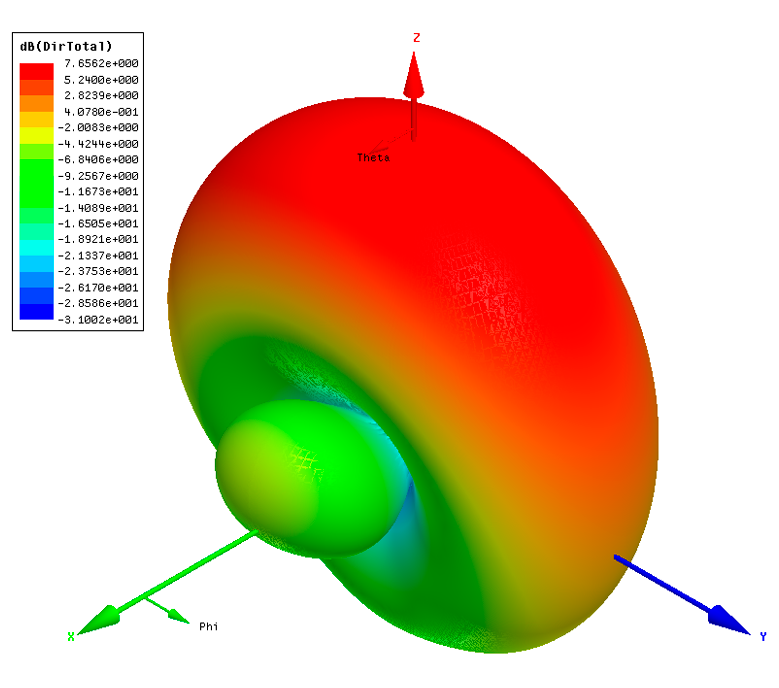
\includegraphics[width=0.85\textwidth]{archivos/analisis/2x11/6}
         \caption{Representación isométrica del diagrama de radiación 3D}
         \label{fig:3d12x11}
     \end{subfigure}
     \hfill
     \begin{subfigure}[b]{0.7\textwidth}
         \centering
         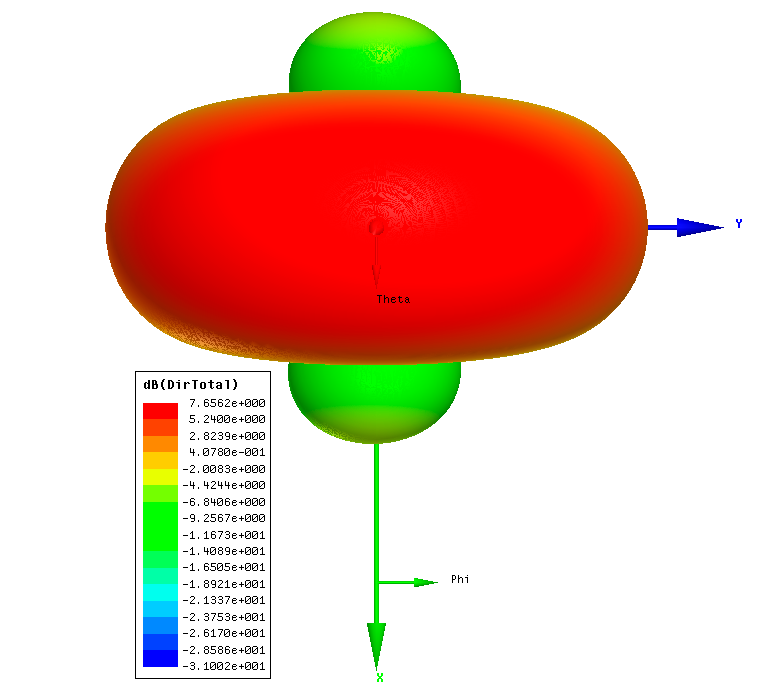
\includegraphics[width=0.85\textwidth]{archivos/analisis/2x11/7}
         \caption{Representación superior del diagrama de radiación 3D}
         \label{fig:3d22x11}
     \end{subfigure}
     \hfill
        \caption{Radiación 3D para el array 2x1 a 2.4 GHz}
        \label{fig:3d2x11}
\end{figure}

\subsection{Campo eléctrico}
\par Finalmente, podemos observar la distribución de campos eléctricos en el parche. 

\begin{figure}[H]
    \centering
        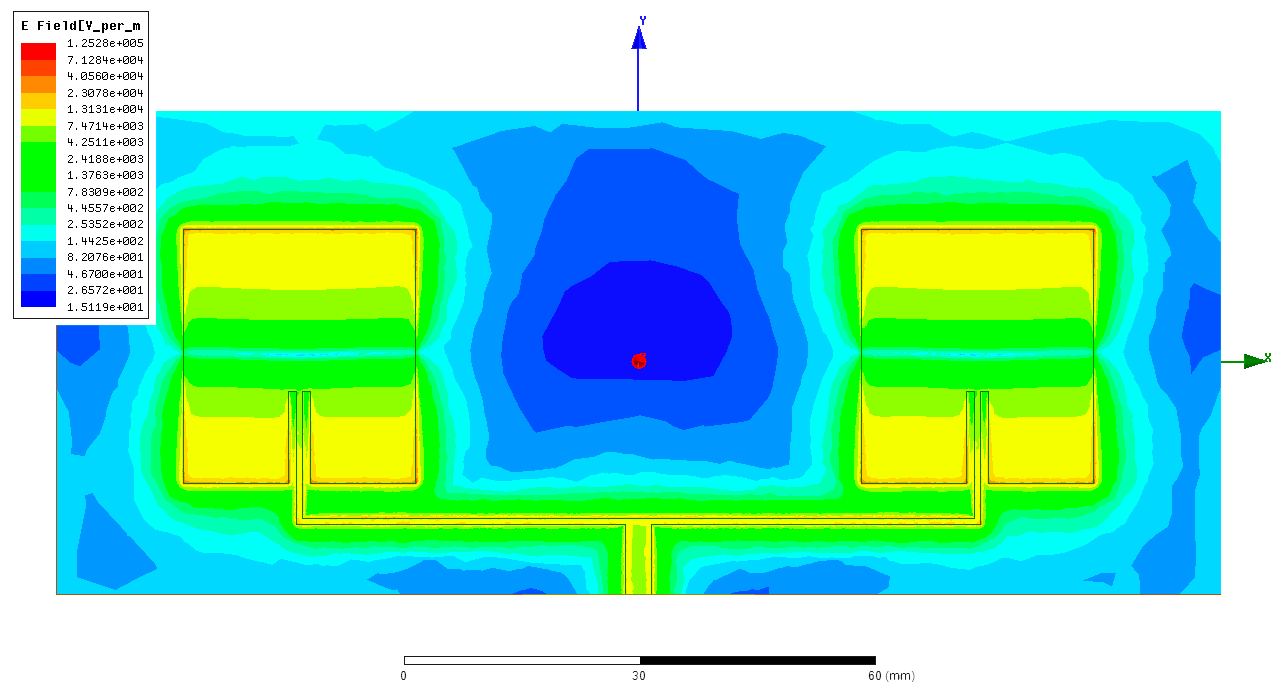
\includegraphics[width=\textwidth]{archivos/analisis/2x11/8}
        \caption{Distribución de campos eléctricos para el para el array 2x1 a 2.4 GHz}
        \label{fig:elec2x11}
\end{figure}

\subsection{Resumen}
\par En esta primera configuración de array a 2.4 GHz se puede observar los primeros comportamientos directivos producidos por la conjunción de diferentes parches en fase funcionando en la misma antena. 
\\
\par En la tabla \ref{tab:2x11} se pueden observar un resumen de los parámetros característicos de la antena. Como se puede observar, el rendimiento obtenido para esta antena es un tanto menor al obtenido previamente en las antenas de parche único y esto es principalmente debido a la complejidad del proceso de adaptación al aumentar el número de parches en las configuraciones de array.

\begin{table}[H]
  
   
   \small % text size of table content
   \centering % center the table
   \begin{tabular}{m{0.2\linewidth}m{0.25\linewidth}} % alignment of each column data
   \toprule[\heavyrulewidth]\toprule[\heavyrulewidth]
   \textbf{Parámetro} & \textbf{Array 2x1 a 2.4 GHz} \\ 
   \midrule
   \textbf{S(1,1)} & -36.46 dB \\
   \textbf{Ancho de banda} & 34.3 MHz dB \\
   \textbf{Directividad} & 7.64 dB \\
   \textbf{Ganancia} & 7.03 dB \\
   \textbf{Eficiencia de radiación} & 86.94\% \\
   \textbf{Relación delante/atrás} & 15.89 dB \\

   \bottomrule[\heavyrulewidth] 
   \end{tabular}
   \label{tab:2x11}
   \caption{Parámetros característicos para el array 2x1 a 2.4 GHz} 
\end{table}













\section{Array 2x1 a 6 GHz}
\par Para el array en configuración 2x1 a 6 GHz los resultados obtenidos son los siguientes:

\subsection{Pérdidas de retorno}
\par En cuanto a su curva de pérdidas de retorno del array a 6 GHz, se puede observar un valor pico de -76.78 dB y un ancho de banda de 179.1 MHz, desde los 5.9014 GHz hasta los 6.0805 GHz, lo que equivale a un 2.98\% de la frecuencia de trabajo.
\\
\begin{figure}[H]
    \centering
        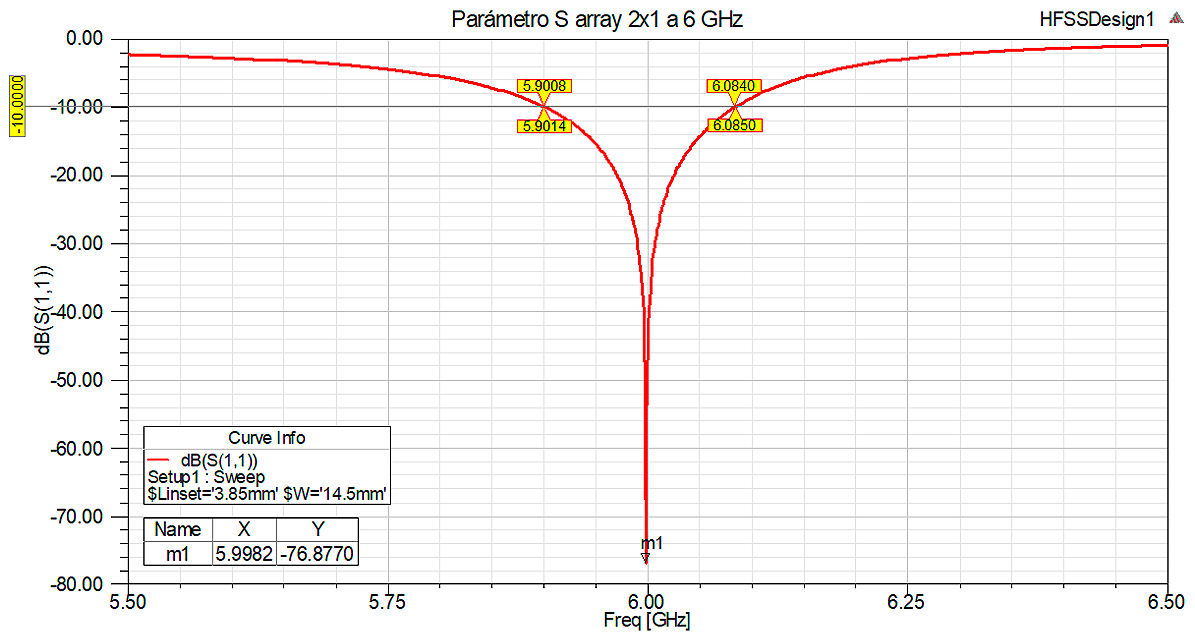
\includegraphics[width=\textwidth]{archivos/analisis/2x12/1}
        \caption{Parámetro S para el array 2x1 a 6 GHz}
        \label{fig:s2x12}
\end{figure}

\newpage
\subsection{Reactancia}
\par La curva de reactancia arroja un valor a la frecuencia de trabajo de -0.03 $\Omega$. 
\\
\begin{figure}[H]
    \centering
        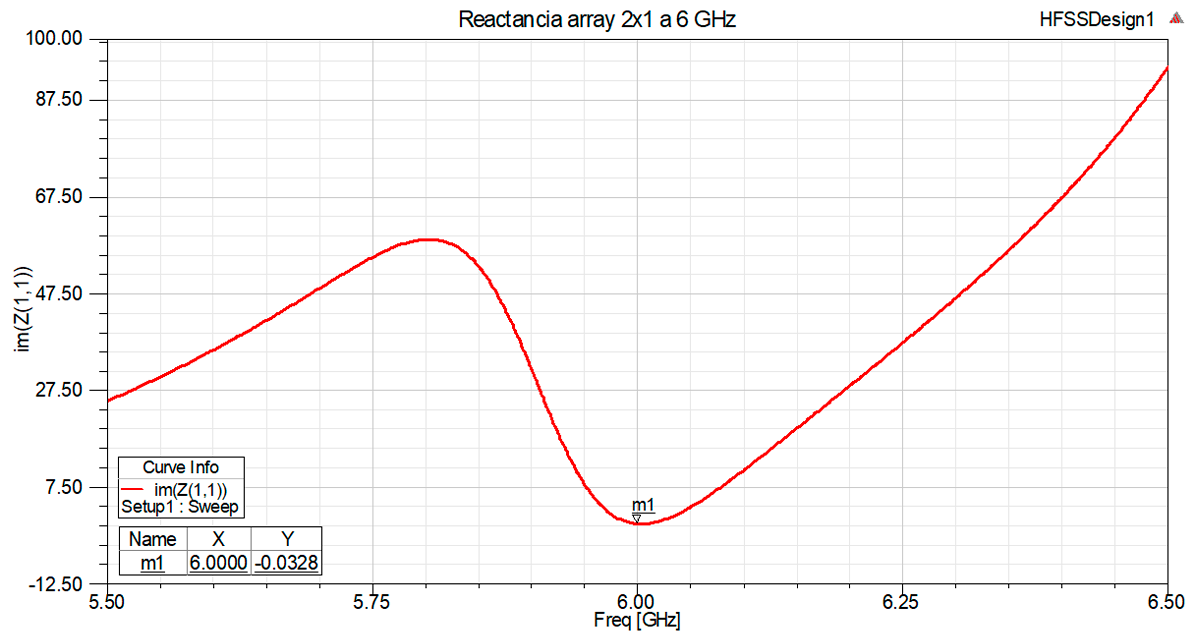
\includegraphics[width=0.85\textwidth]{archivos/analisis/2x12/2}
        \caption{Reactancia para el array 2x1 a 6 GHz}
        \label{fig:react2x12}
\end{figure}

\subsection{Resistencia}
\par La parte real de la impedancia ofrece un valor a la frecuencia de trabajo de 49.35 $\Omega$.
\\
\begin{figure}[H]
    \centering
        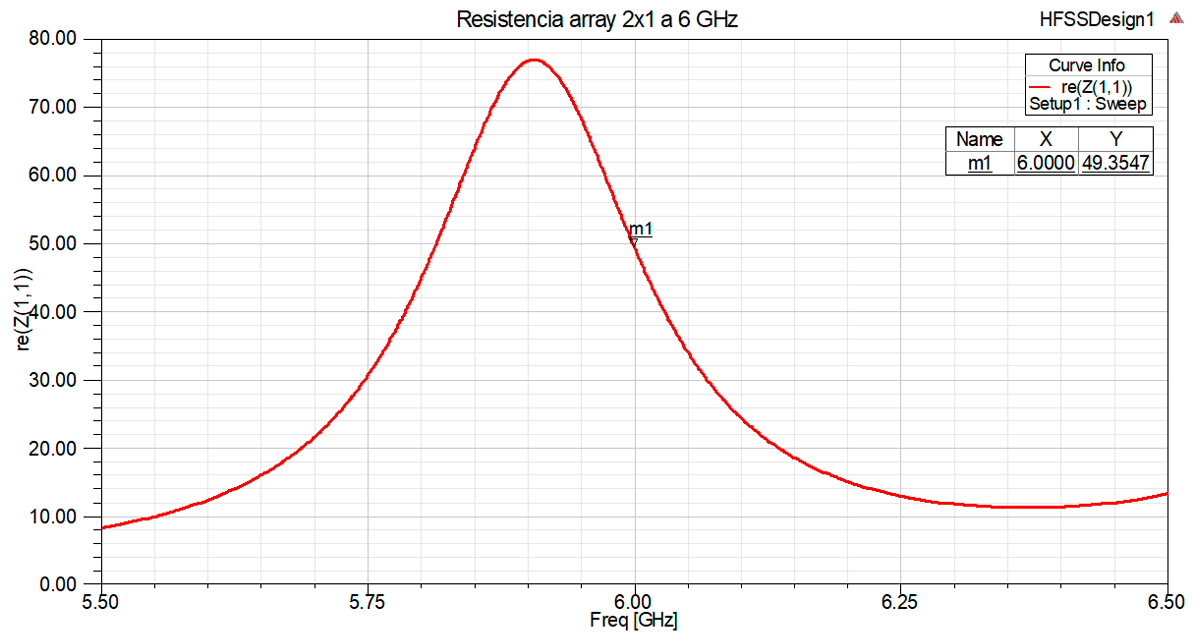
\includegraphics[width=0.85\textwidth]{archivos/analisis/2x12/3}
        \caption{Resistencia para el array 2x1 a 6 GHz}
        \label{fig:resis2x12}
\end{figure}

\subsection{Patrón de radiación}
\par En este caso se puede observar el mismo patrón de radiación base que se encontró en el array 2x1 a 2.4 GHz pero con una directividad aumentada del lóbulo principal con respecto a los lóbulos secundarios y traseros, con un pico de directividad en el ángulo de máxima radiación de 9.97 dB. 
\\
\subsubsection{Plano E}
\begin{figure}[H]
    \centering
        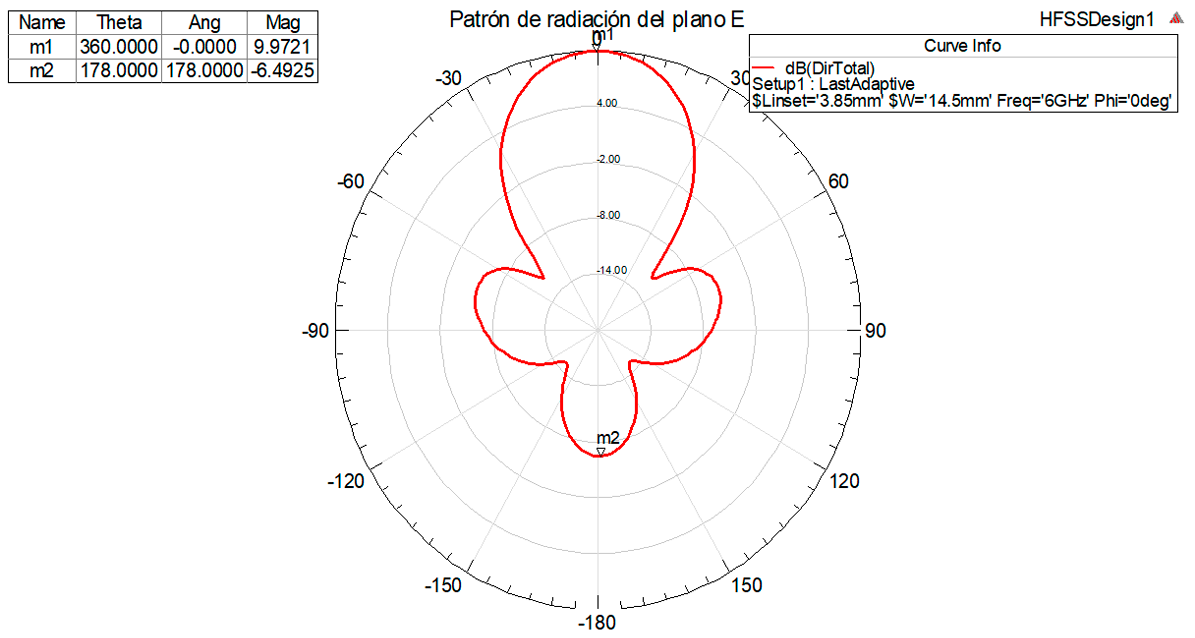
\includegraphics[width=0.8\textwidth]{archivos/analisis/2x12/4}
        \caption{Radiación en el plano E para el array 2x1 a 6 GHz}
        \label{fig:E2x12}
\end{figure}

\subsubsection{Plano H}
\begin{figure}[H]
    \centering
        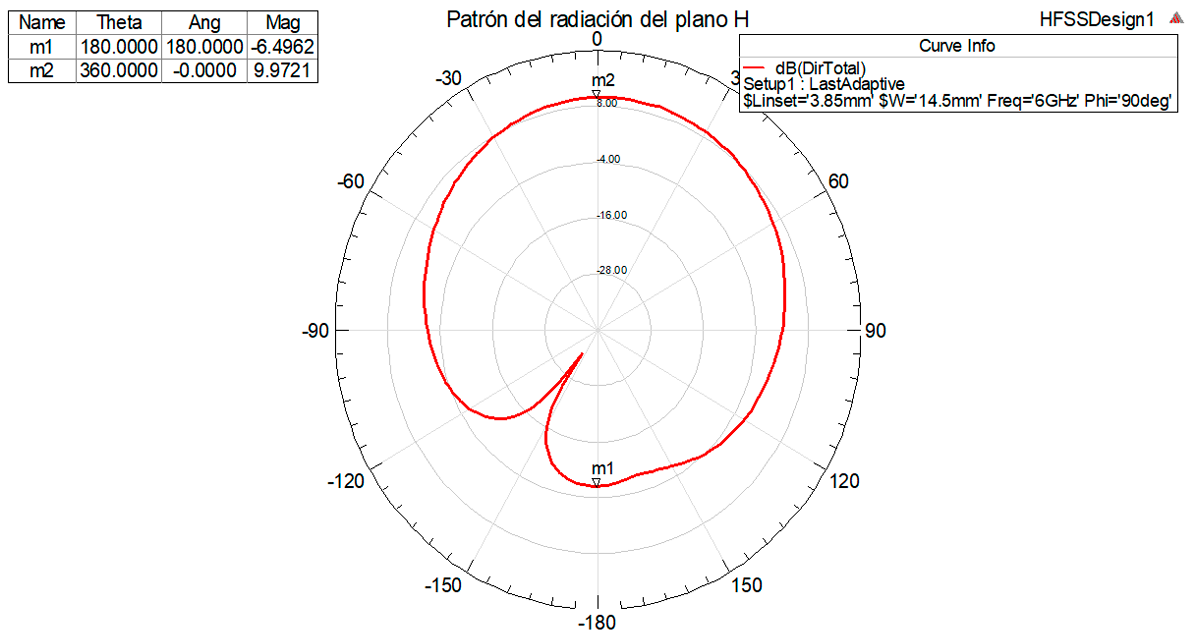
\includegraphics[width=0.8\textwidth]{archivos/analisis/2x12/5}
        \caption{Radiación en el plano H para el array 2x1 a 6 GHz}
        \label{fig:H2x12}
\end{figure}

\subsection{Radiación 3D}
\par Mediante el diagrama de radiación 3D se puede observar, de nuevo, el mismo comportamiento directivo que encontramos en el array a 2.4 GHz de la misma configuración, pero con ese aumento de directividad sobre el lóbulo principal, dejando a los lóbulos laterales en un segundo plano en cuanto a la radiación que estos ofrecen.

\begin{figure}[H]
     \centering
     \begin{subfigure}[b]{0.7\textwidth}
         \centering
         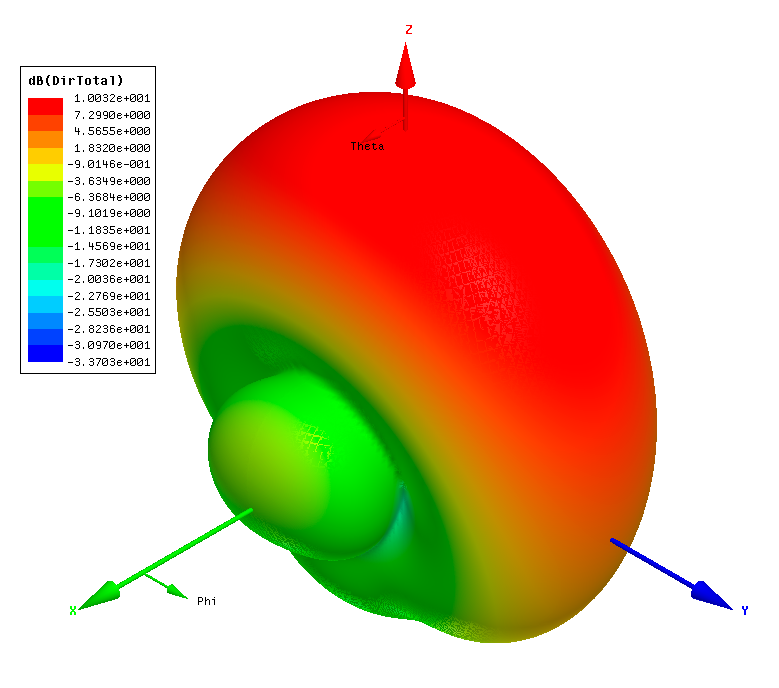
\includegraphics[width=0.85\textwidth]{archivos/analisis/2x12/6}
         \caption{Representación isométrica del diagrama de radiación 3D}
         \label{fig:3d12x12}
     \end{subfigure}
     \hfill
     \begin{subfigure}[b]{0.7\textwidth}
         \centering
         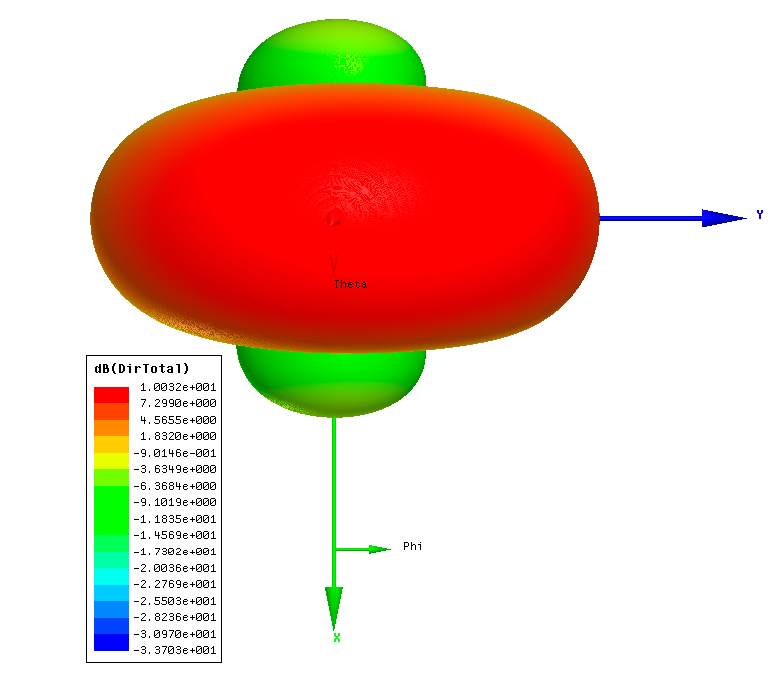
\includegraphics[width=0.85\textwidth]{archivos/analisis/2x12/7}
         \caption{Representación superior del diagrama de radiación 3D}
         \label{fig:3d22x12}
     \end{subfigure}
     \hfill
        \caption{Radiación 3D para el array 2x1 a 6 GHz}
        \label{fig:3d2x12}
\end{figure}

\subsection{Campo eléctrico}
\par Finalmente, podemos observar la distribución de campos eléctricos en el parche. 

\begin{figure}[H]
    \centering
        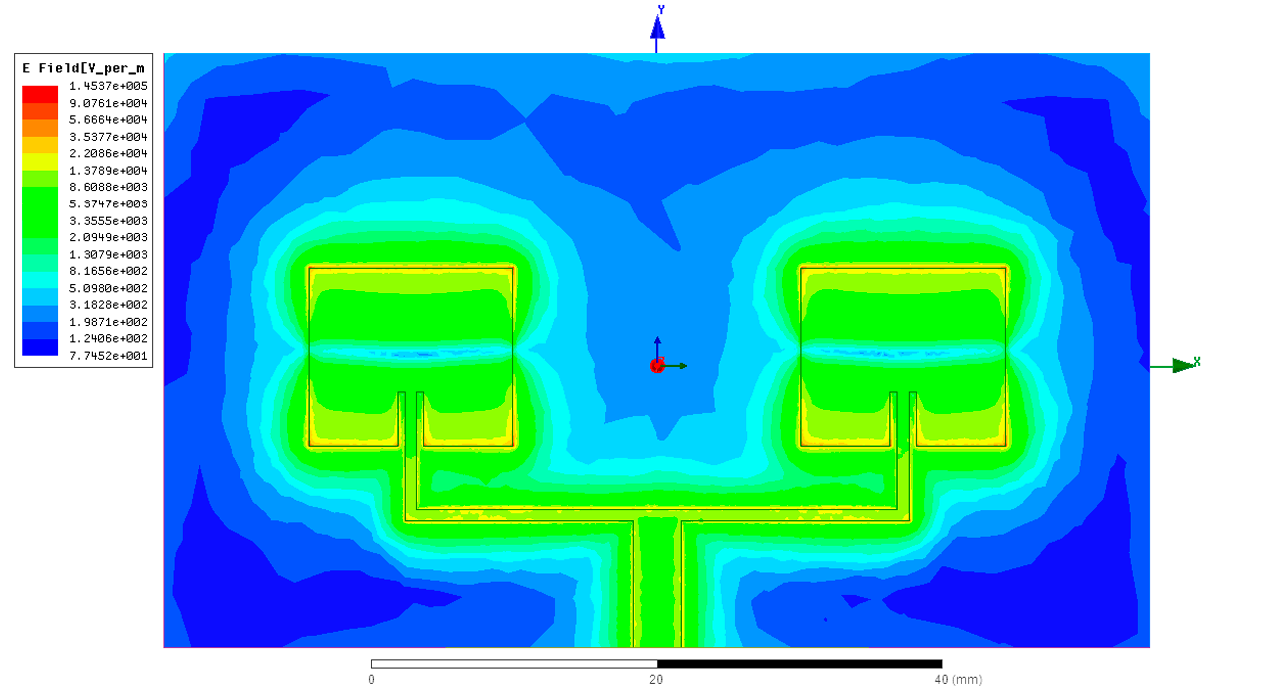
\includegraphics[width=\textwidth]{archivos/analisis/2x12/8}
        \caption{Distribución de campos eléctricos para el para el array 2x1 a 6 GHz}
        \label{fig:elec2x12}
\end{figure}

\subsection{Resumen}
\par En la configuración 2x1 a 6 GHz se puede observar una mejora de parámetros característicos de la antena con respecto a los obtenidos para la antena de 2.4 GHz en la misma configuración. Esto es principalmente debido a la mejor adaptación que ha tenido esta antena entre el conjunto de líneas microstrip que la alimentan.
\\
\par En la tabla \ref{tab:2x12} se pueden observar un resumen de los parámetros característicos de la antena.

\begin{table}[H]
  
   
   \small % text size of table content
   \centering % center the table
   \begin{tabular}{m{0.2\linewidth}m{0.25\linewidth}} % alignment of each column data
   \toprule[\heavyrulewidth]\toprule[\heavyrulewidth]
   \textbf{Parámetro} & \textbf{Array 2x1 a 6 GHz} \\ 
   \midrule
   \textbf{S(1,1)} & -76.87 dB \\
   \textbf{Ancho de banda} & 179.1 MHz dB \\
   \textbf{Directividad} & 9.97 dB \\
   \textbf{Ganancia} & 9.77 dB \\
   \textbf{Eficiencia de radiación} & 94.14\% \\
   \textbf{Relación delante/atrás} & 16.64 dB \\

   \bottomrule[\heavyrulewidth] 
   \end{tabular}
   
   \caption{Parámetros característicos del array 2x1 a 6 GHz} 
   \label{tab:2x12}
\end{table}


















\section{Array 2x2 a 2.4 GHz}
\par Para el array en configuración 2x2 a 2.4 GHz los resultados obtenidos son los siguientes:

\subsection{Pérdidas de retorno}
\par En cuanto a su curva de pérdidas de retorno del array a 2.4 GHz, se puede observar un valor pico de -76.78 dB y un ancho de banda de 179.1 MHz, desde los 5.9014 GHz hasta los 6.0805 GHz, lo que equivale a un 2.98\% de la frecuencia de trabajo.
\\
\begin{figure}[H]
    \centering
        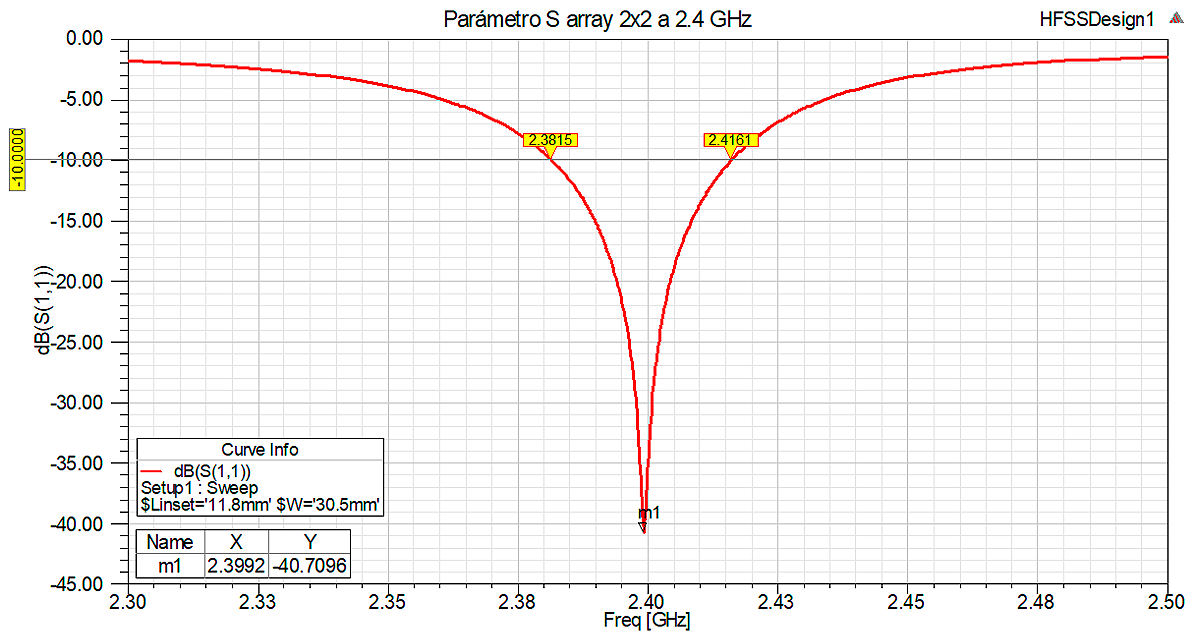
\includegraphics[width=\textwidth]{archivos/analisis/2x21/1}
        \caption{Parámetro S para el array 2x2 a 2.4 GHz}
        \label{fig:s2x21}
\end{figure}

\newpage
\subsection{Reactancia}
\par La curva de reactancia arroja un valor a la frecuencia de trabajo de -0.03 $\Omega$. 
\\
\begin{figure}[H]
    \centering
        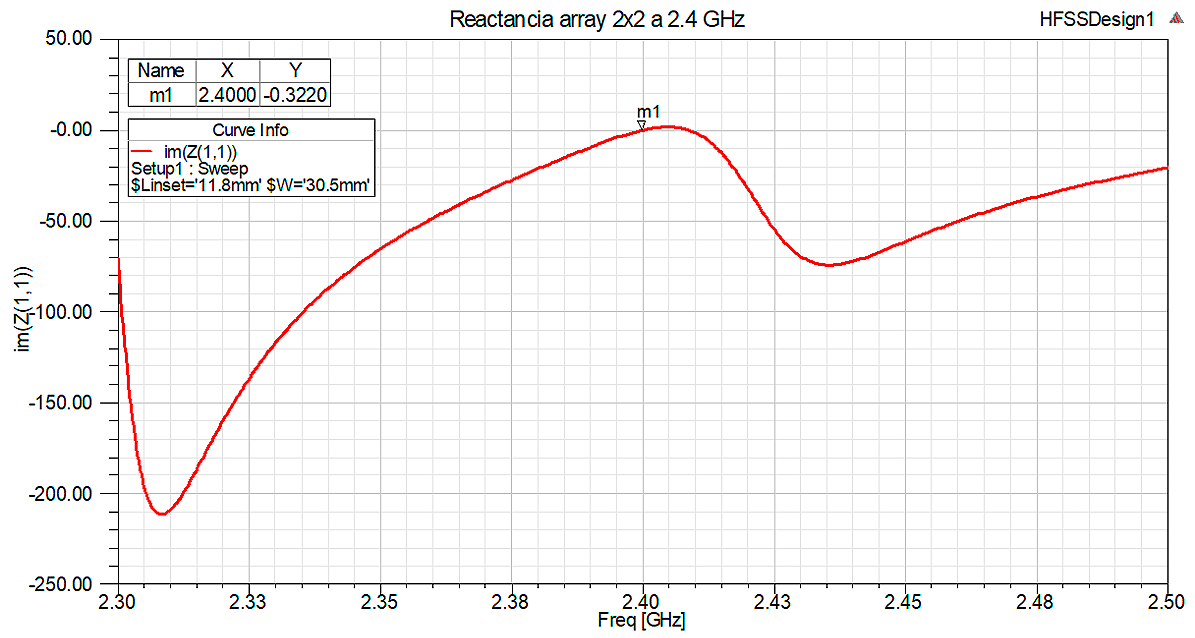
\includegraphics[width=0.8\textwidth]{archivos/analisis/2x21/2}
        \caption{Reactancia para el array 2x2 a 2.4 GHz}
        \label{fig:react2x21}
\end{figure}

\subsection{Resistencia}
\par La parte real de la impedancia ofrece un valor a la frecuencia de trabajo de 49.35 $\Omega$.
\\
\begin{figure}[H]
    \centering
        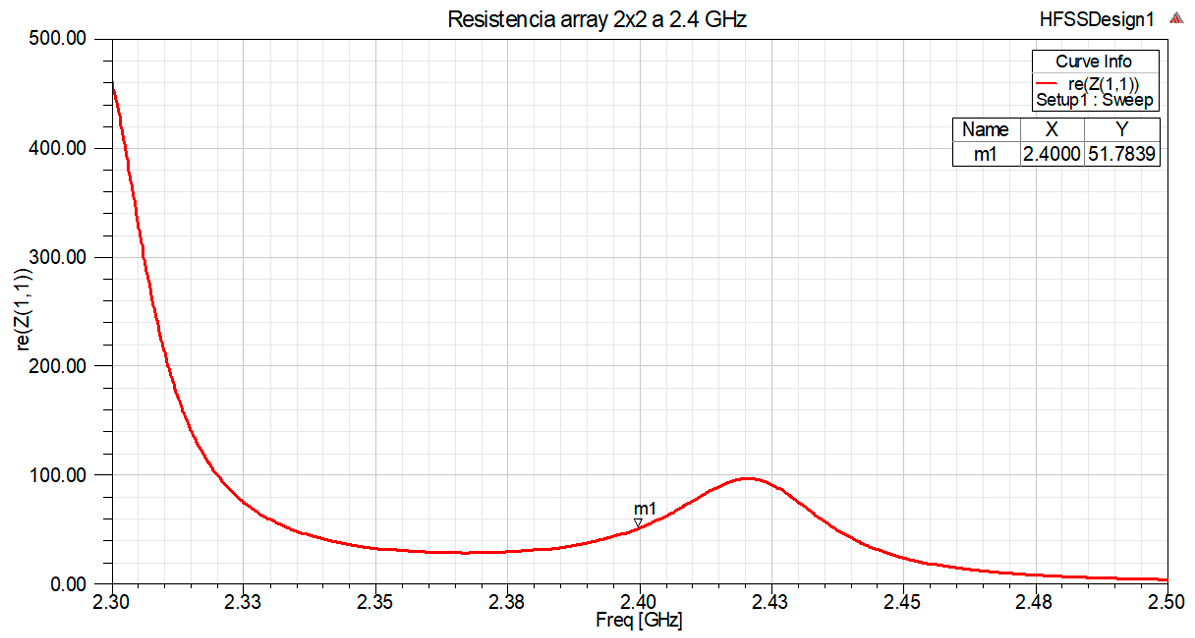
\includegraphics[width=0.8\textwidth]{archivos/analisis/2x21/3}
        \caption{Resistencia para el array 2x2 a 2.4 GHz}
        \label{fig:resis2x21}
\end{figure}

\subsection{Patrón de radiación}
\par En este caso se puede observar el mismo patrón de radiación base que se encontró en el array 2x2 a 2.4 GHz pero con una directividad aumentada del lóbulo principal con respecto a los lóbulos secundarios y traseros, con un pico de directividad en el ángulo de máxima radiación de 9.97 dB. 
\\
\subsubsection{Plano E}
\begin{figure}[H]
    \centering
        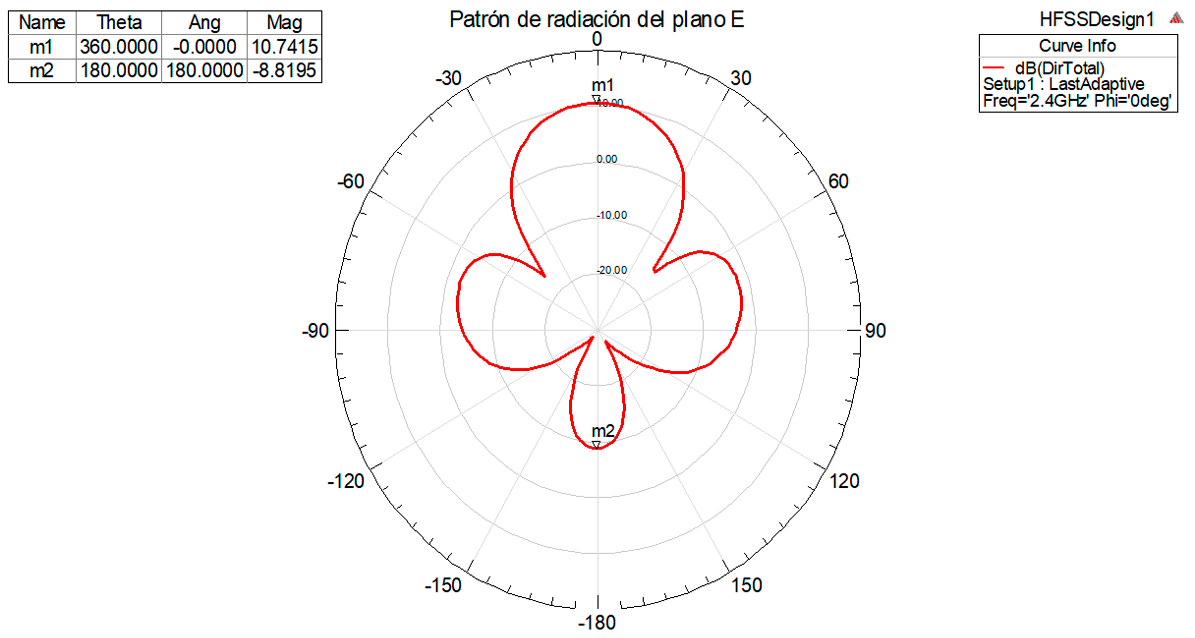
\includegraphics[width=0.8\textwidth]{archivos/analisis/2x21/4}
        \caption{Radiación en el plano E para el array 2x2 a 2.4 GHz}
        \label{fig:E2x21}
\end{figure}

\subsubsection{Plano H}
\begin{figure}[H]
    \centering
        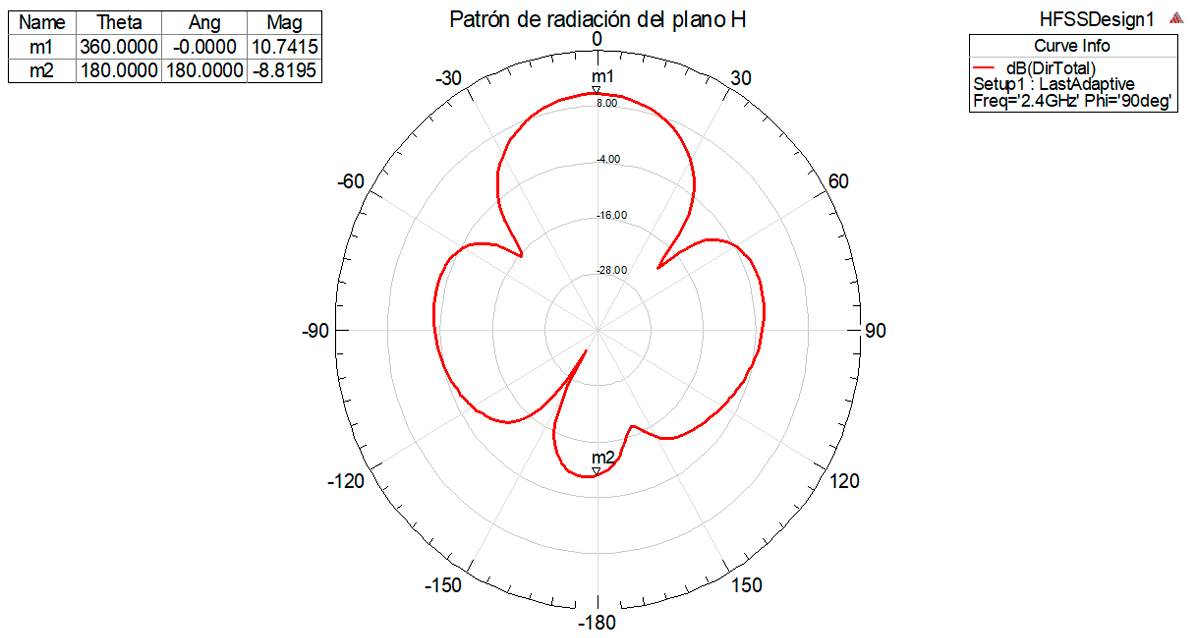
\includegraphics[width=0.8\textwidth]{archivos/analisis/2x21/5}
        \caption{Radiación en el plano H para el array 2x2 a 2.4 GHz}
        \label{fig:H2x21}
\end{figure}

\subsection{Radiación 3D}
\par Mediante el diagrama de radiación 3D se puede observar, de nuevo, el mismo comportamiento directivo que encontramos en el array a 2.4 GHz de la misma configuración, pero con ese aumento de directividad sobre el lóbulo principal, dejando a los lóbulos laterales en un segundo plano en cuanto a la radiación que estos ofrecen.

\begin{figure}[H]
     \centering
     \begin{subfigure}[b]{0.7\textwidth}
         \centering
         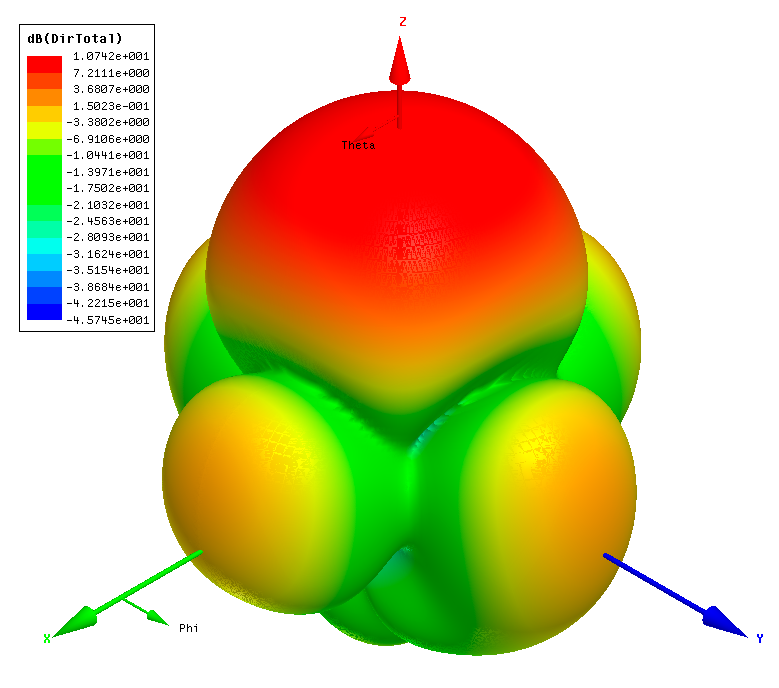
\includegraphics[width=0.85\textwidth]{archivos/analisis/2x21/6}
         \caption{Representación isométrica del diagrama de radiación 3D}
         \label{fig:3d12x21}
     \end{subfigure}
     \hfill
     \begin{subfigure}[b]{0.7\textwidth}
         \centering
         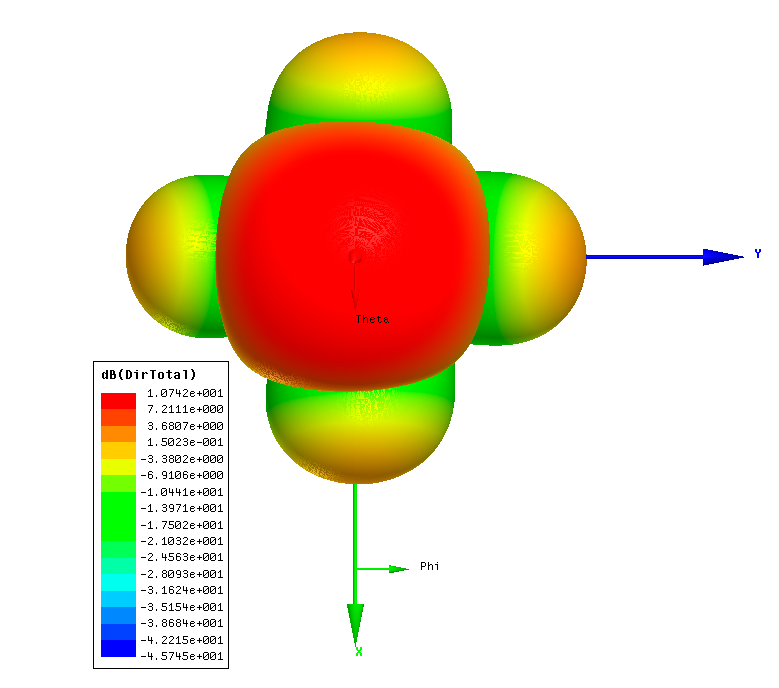
\includegraphics[width=0.85\textwidth]{archivos/analisis/2x21/7}
         \caption{Representación superior del diagrama de radiación 3D}
         \label{fig:3d22x21}
     \end{subfigure}
     \hfill
        \caption{Radiación 3D para el array 2x2 a 2.4 GHz}
        \label{fig:3d2x21}
\end{figure}

\subsection{Campo eléctrico}
\par Finalmente, podemos observar la distribución de campos eléctricos en el parche. 

\begin{figure}[H]
    \centering
        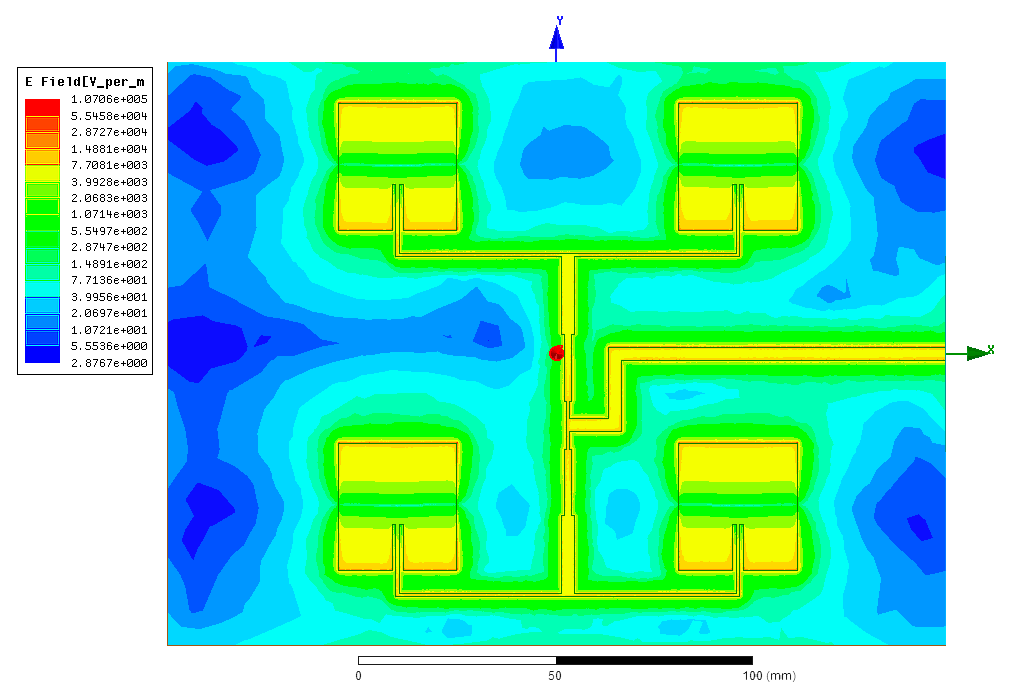
\includegraphics[width=\textwidth]{archivos/analisis/2x21/8}
        \caption{Distribución de campos eléctricos para el para el array 2x2 a 2.4 GHz}
        \label{fig:elec2x21}
\end{figure}

\subsection{Resumen}
\par En la configuración 2x2 a 2.4 GHz se puede observar una mejora de parámetros característicos de la antena con respecto a los obtenidos para la antena de 2.4 GHz en la misma configuración. Esto es principalmente debido a la mejor adaptación que ha tenido esta antena entre el conjunto de líneas microstrip que la alimentan.
\\
\par En la tabla \ref{tab:2x21} se pueden observar un resumen de los parámetros característicos de la antena.

\begin{table}[H]
  
   
   \small % text size of table content
   \centering % center the table
   \begin{tabular}{m{0.2\linewidth}m{0.25\linewidth}} % alignment of each column data
   \toprule[\heavyrulewidth]\toprule[\heavyrulewidth]
   \textbf{Parámetro} & \textbf{Array 2x2 a 2.4 GHz} \\ 
   \midrule
   \textbf{S(1,1)} & -76.87 dB \\
   \textbf{Ancho de banda} & 179.1 MHz dB \\
   \textbf{Directividad} & 9.97 dB \\
   \textbf{Ganancia} & 9.77 dB \\
   \textbf{Eficiencia de radiación} & 94.14\% \\
   \textbf{Relación delante/atrás} & 16.64 dB \\

   \bottomrule[\heavyrulewidth] 
   \end{tabular}
   
   \caption{Parámetros característicos del array 2x2 a 2.4 GHz} 
   \label{tab:2x21}
\end{table}







